\chapter{MagicDrawToGamma plugin}


\section{Koncepció}
Állapottérképek formális verifikációjának támogatása MagicDraw-ban, egy plug-in fejlesztésével lett megvalósítva. A plug-in függ a Viatra For MagicDraw-tól, ami lehetővé teszi modellek transzformációját Viatra segítségével. A plug-in legfontosabb funkciója MagicDraw modellek Gamma modellekké való transzformációja. A letranszformált Gamma nyelvű modelleket az keretrendszer kezelni tudja, a verifikáció elvégzéséhez az eszköznek csak egyes részei szükségesek. A megoldást a \ref{fig:used-gamma} ábra szemlélteti. A felhasználónak lehetősége van megkötések megfogalmazására a plugin-al és elvégezni a verifikációt és megtekinteni az eredményt azaz, hogy teljesülnek-e a megkötések vagy sem.

\begin{figure}[!ht]
	\centering
	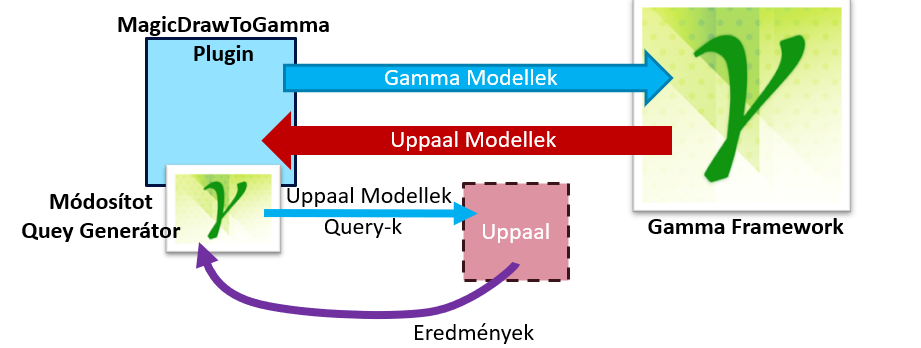
\includegraphics[keepaspectratio, width=150mm]{figures/concept.png}
	\caption{Koncepció}
	\label{fig:used-gamma}
\end{figure}

\section{Fejlesztőkörnyezet}
 A fejlesztés megkezdéséhez szükséges volt összeállítani egy olyan fejlesztőkörnyezetet amivel hatékonyan lehet plug-int fejleszteni. MagicDraw biztosít egy ún. \emph{skeletont} Eclipsehez és IntelliJhez is plug-in fejlesztéséhez, de a fejlesztés nem ezek segítségével hanem az IncQueryLabs által készített skeleton felhasználásával valósult meg. Ennek oka, hogy a hivatalos \emph{skeletonok} nem vagy csak részben működtek, a mögöttes infrastruktúra megismerése és javítása pedig túl hosszadalmas és a feladat szempontjából irreleváns lett volna. 
 
A skeleton egy Eclipse project, viszont Gradlet használ a projekt fordításához és a dependenciák kezeléséhez. Ez sokszor inkonzisztenciákhoz vezetett az egyik legnagyobb probléma a Viatra Querik generálása csak Eclipsel lehet generálni. A kódbázis egy része nem Javában hanem Xtendben íródott, a Viatra modell transzformációk implementálása ezzel a nyelvvel egyszerűbb. Azok az osztályok melyeknél nem volt indokolt, jellemzően a MagicDraw felhasználói felületeinél, azok Java 8-ban lettek implementálva.

A dolgozat elkészítése idején a MagicDraw 19-es verziója is elérhető volt a plug-in azonban még nem ehhez, hanem a 18.5-ös verziójához készült. A kódbázis azonban kompatibilis lehet még az újabb verziókkal is, amennyiben az állapottérképeket érintő meta-modellek nem változnak.

Gamma(2.0) a verifikációt Uppaal segítségével végzi el. Ehhez előállít egy leírást a rendszerről és egy queryt ami a rendszerrel szemben támasztott követelményeket írja le. Utóbbi megírásához biztosít egy UI elemet amivel a felhasználó az Uppaal ismerete nélkül is képes a követelmények definiálására. Ez a funkció teljesen át lett emelve Gammából módosított implementációval a MagicDrawToGammába. A Gamma az Uppaalra az operációs rendszeren keresztül hív át, ezért az Uppaalt külön kell telepíteni és konfigurálni.

\section{MagicDraw - Gamma transzformáció}

A MagicDraw - Gamma transzfromációt egy menü elemmel lehet elindítani. Ehhez szükséges, hogy a projekthez hozzá legyen rendelve egy külső könyvtár (Gamma Workspace) ami a leképzett és perzisztensen eltárolandó modellek helyét jelöli. A hozzárendelt könyvtár abszolút elérését String formában a projekt tárolja, emiatt sem a projekt nem migrálható, sem pedig maga a Gamma Workspace. Továbbá a könyvtár karbantartása ebben a verzióban még a felhasználó felelőssége, ugyanis a plug-in nem töröl a könyvtárból csak hozzáad és módosít, ennek akkor van jelentősége, ha leképzés után egy állapottérkép el lett távolítva a MagicDraw modellből és utána újra le lett képezve. Ebben az esetben a régebben leképzett Gamma állapottérképek is megmaradnak.

\subsection{Gyökér elemek létrehozása:}

A plugin a transzformáió elején létrehoz egy \emph{ResourceSet}-et, amibe készít egy \emph{Resource}-t a \emph{Gamma Workpace} gyökerébe .s.md2g néven, továbbá egy Resource-t \verb+interfaces.gms+ néven. Az előbbi Resource egy segédstruktúrát tartalmaz ami a leképzett elemek visszakereshetőségéül szolgál (ld. \refstruc{sec:trace_model}), utóbbi pedig a modellben definiált interfaceket tárolja.

Az eszköz ezután Viatra Queryk segítségével megkeresi az állapotgépeket a MagicDrawban és végig iterál rajtuk. Minden állapottérképen kigyűjti az éleken használt Signal Eventeket és létrehoz a Signaléval azonos néven egy Eventet, a Gamma meta-modelljének megfelelően. A létrehozott eventek egy Interfacen kerülnek definiálásra aminek a neve megegyezik az állapottérképével. Az interface ezután belekerül az interfaceket tároló \emph{Resourceba}. Az eventek iránya INOUT ez lehetővé teszi azt is, hogy az állapotgép magának küldjön eseményt.

A leképzett állapottérképek külön Resourceokba kerülnek amik a Gamma Workspace-ben egy külön az állapottérkép nevével megegyező könyvtárba kerülnek, ugyan ezen a néven .gsm kiterjesztéssel (\ref{fig:filestructure}-es ábra). (A Resource gyökere nem egy StatechartDefinition, hanem egy Package, ennek a neve szintén megegyezik az állapottérkép nevével)

\begin{figure}[H]
	\centering
	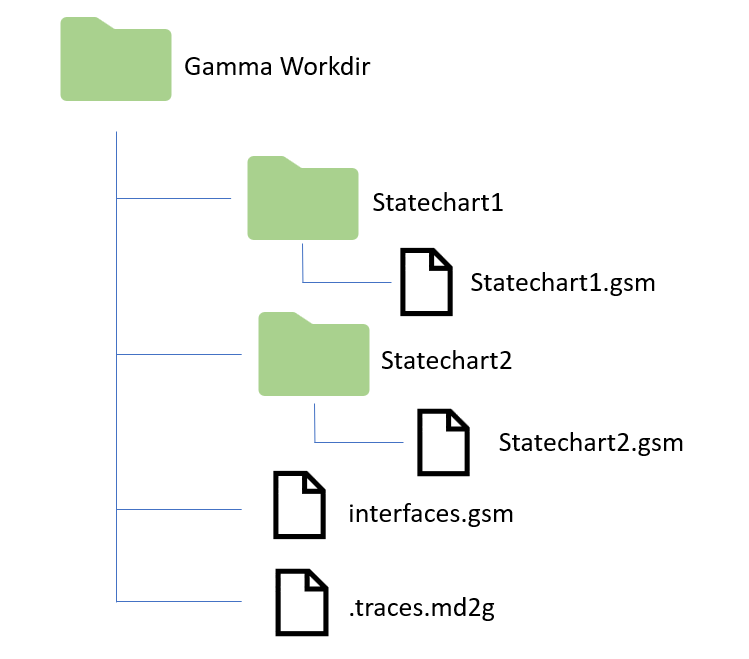
\includegraphics[keepaspectratio, width=90mm]{figures/filestructure.png}
	\caption{Létrehozott fájlstruktúra}
	\label{fig:filestructure}
\end{figure}

\subsection{Alap struktúra kialakítása:}

Az előző lépések során azok az elemek állnak elő, melyek a modellek gyökér elemeiként fognak szolgálni. A következő lépés létrehozni az állapottérképek egy belső, alap struktúráját, amit az állapotok és állapotátmenetek határoznak meg. A Viatra for MagicDraw projekt megnyitásakor készít egy ViatraQueryEngine-t aminek a Scope-ja a megnyitott modellre terjed ki. A transzformációs szabályok regisztrálása ezen az engine-en történik, létrejön azonban még egy aminek a Scope-ja magába foglalja az első lépésben lérehozott \emph{Resource}okat és a MagicDraw modellt is. A készülő modellben történő keresések, és a visszakövetések ezzel az engine-el történnek. Alap struktúra kialakításának lépcsői:

\begin{enumerate}
	\item Fő régiók leképzése (olyan régió aminek a szülője állapotgép).
	\label{enum:elso}
	\item Régiókban található állapotok leképzése.
	\label{enum:masodik}
	\item Állapotokban található régiók leképzése.
	\label{enum:harmadik}
\end{enumerate}


A második lépésben a Trace Modell alapján megkeressük a már leképzett régiót a Gamma Modellben és beletesszük az újonnan létrehozott és a MagicDraw modellnek megfelelően elnevezett állapotot, ha a régió még nincs leképezve akkor létrejön, és abba kerül bele az állapotot. Ez a lépés olyan részgráfokat is eredményezhet amikbe nem vezet út a gyökér elemekből. Ennek kiküszöbölése a harmadik. lépés ami, ugyan ezt a műveletet hajtja végre csak a másik irányból, tehát az állapotok párjait keressük meg, amikbe régiókat helyezünk el. Ezek a régiók már létezhetnek ilyenkor nem új régió jön létre hanem a már meglévő kerül az állapotba. A működés során a MagicDraw modell jól formáltsága kihasznált és elvárt, továbbá az is ki van használva, hogy régió csak \emph{State}ben és Állapotgépben lehet. A régiókat tartalmazó állapotok kompozit és ortogonális állapotnak tekintendők.

A tartalmazási gráf összefüggővé válását \aref{fig:state-transformation} ábra szemlélteti.

\begin{figure}[H]
Az irányított nyilak tartalmazást jelölnek, a bekeretezett téglalap StatechartDefinition, a szagatott vonallal körbevett Region és a körök Statek.

\centering
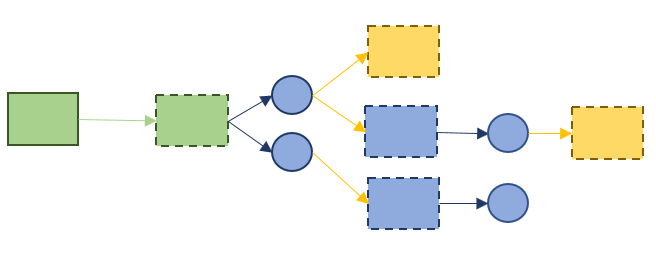
\includegraphics[keepaspectratio, width=140mm]{figures/transformation.png}
\caption{Állapotok és régiók leképzésének menete, \ref{enum:elso}. lépcső: zöld, \ref{enum:masodik}. lépcső: kék, \ref{enum:harmadik}. lépcső: sárga}
\label{fig:state-transformation}
\end{figure}


\subsection{Pszeudoállapotok átalakítása:}
Az állapotátmenetek leképzése előtt a pszeudoállapotok kerülnek leképzésre. Ezen a ponton már létezik minden régió amit tartalmazhatja őket. A leképzés legtöbb esetben támogatott viszont, egyes elemek tartalmazása esetén nem lehet a verifikációt végrehajtani. Az elemeket és párjaikat \aref{table:pseudo} táblázat mutatja.

\begin{table}[!h]
	\footnotesize
	\centering
	\begin{tabular}{ l c c }
		MagicDraw & Gamma & verifikálható \\ \hline
		InitialState & InitialState & igen \\
		Chioce & Choice & igen \\
		Junction & Merge & nem \\
		Fork & Fork & nem \\
		Join & Join & nem \\
		TerminalState & nincs & - \\
		Conn. PointReference & nincs & - \\
		EntryPoint & nincs & - \\
		ExitPoint & nincs & -
		
	\end{tabular}
	\caption{Pszeudoállapotok párosítása.}
	\label{table:pseudo}
\end{table}

\subsection{Állapotátmenetek leképzése:} A következő lépés az állapotátmenetek átalakítása. Ezen a ponton már az összes olyan elem leképzésre került, amely az állapotátmenetek kezdő, vagy végpontjaként szolgálhat. Egy MagicDraw modellben az állapotátmenetek régiók tartalmazzák, szemben Gammával, ahol a StatechartDefinition közvetlen gyerekei. A tartalmazó-tartalmazott, Statemahcine - Tranisiton párok megkeresése a következő patternekkel történik.
\lstset{style=VQL}
\begin{lstlisting}
pattern RegionsInRegion(container: Region, region: Region){
	Region.subvertex(container, vertex);
	State.region(vertex, region);
}
pattern RegionsInStatemachine(stateMachine: StateMachine, subregion: Region){
	find MainRegions(stateMachine, subregion);
} or {
	find RegionsInRegion+(region, subregion);
	StateMachine.region(stateMachine, region);
}
pattern TranisitonsInStateMachine(stateMachine: StateMachine, transition: Transition){
	find RegionsInStatemachine(stateMachine, region);
	Region.transition(region, transition);
}
\end{lstlisting}

A StateMachine Gamma modellbeli párját a \emph{Trace modell} segítségével lehet megtalálni és hozzáadni a megfelelő állapotátmenetet.

Az átmenetek leképzése után már elérhetőséget lehet is vizsgálni.

\subparagraph{Változók leképzése}
Változókat MagicDraw-ben attribútumként van lehetősége definiálni. FOLYT
%TODO FOLYT


\subsection{Triggerek leképzése:} A MagicDrawban definiálható \emph{Triggerek} pontosabban az őket kiváltó események közül jelenleg kettő támogatott. Egyik a \emph{SignalEvent} a másik pedig \emph{Time Event}. Előbbi \emph{EventTriggerre} képződik le. A felhasználónak a \emph{SignalEvent} forrásával most még nem kell foglalkoznia, hiszen ezekhez automatikusan generálódik egy \emph{Interface} és egy \emph{Port}.

A \emph{Time Eventek} MagicDraw-ban két féle típusúak lehetnek: relatív és abszolút. Utóbbit a plugin-in még nem támogatja.
A relatív típusú \emph{Time Eventek} a Gamma \emph{Timeout} mechanizmusának feleltethető meg. Ez három részből áll: \emph{StatechartDefinition}-ön definiált \emph{TimeoutDeclaration}, akció ami ennek beállítja az értékét (ami lehet szekundumban, vagy milliszekundumban mért) és maga a \emph{Trigger} ami hivatkozik a deklarációra. A \emph{TimeoutDeclaration} és az érték beállítása implicit történik a felhasználónak az időt kell megadnia trigger felvételekor a MagicDraw modellben.

\subsection{Őrfeltételek leképzése:} őrfeltételek definiálása MagicDraw állapottérképeken Opaque Expressionökkel\footnote{Szöveges nyelvel leírt kifejezés} történik, ezért ezt le kell fordítani és modell alapú leírássá konvertálni. Kifejezéseket Gammában a Constraint modellel lehet leírni. Ehhez tartozik egy nyelvtan is ami Xtext segítségével képes a Gamma Constraint nyelvből EMF alapú Constraint Modell példánymodellt fordítani. A MagicDrawToGamma ezen verziója az őrfeltételek leképzéséhez egy saját egyszerűsített implementációt használ. Ennek vannak megkötései is: kifejezések nem ágyazhatók, vagy láncolhatók, változókra és paraméterekre lehet hivatkozni, de csak a gazda StatechartDefinitionban ezen felül csak logikai és Long értékeket lehet használni.

\subsection{Akciók leképzése:} A MagicDraw akciói viselkedések (\emph{Behavior}) lehetnek, ezek leképzését a MagicDrawToGamma nem támogatja, kivéve a \emph{Functional Behavior} viselkedést, amit egy \emph{Opaque Expression} definiál. Ebben kétféle akciót lehet végrehajtani: értékadást és \emph{Signal} küldést. Ezek szintaktikája a következő:

\begin{lstlisting}
	set variableName := 1;
	raise Event
\end{lstlisting}

%TODO FOLYT
FOLYT


\subsection{Trace Modell}
\label{sec:trace_model}
A leképzések végrehajtása során fontos követni, hogy mely elemek képződtek le és mely elemekké. Erre a célra a MagicDrawToGamma bevezet egy Trace modell\footnote{Nem összekeverendő a \aref{sec:formal-verif} fejezetben említett \emph{Execusion Tracel}} nevű segédstruktúrát, ami lehetővé teszi a megfeleltetések visszakereshetőségét Viatrával, továbbá a modell sorosítása és háttértáron való tárolása is megoldott. A modell EMF-ben definiálva és  háromféle \emph{Trace}-t különbötet meg. Az Gamma állapottérképek alap elemeit \verb+Trace+-ek az interfészek elemeit \verb+InterfaceTrace+-k és a \emph{Contraint} modell elemeit \verb+ConstraintTracek+ kötik össze MagicDraw párjukkal, amiből le lettek képezve.

A három \verb+Trace+ típust egy \verb+AbstractTrace+ osztály fogja össze, és \verb+MD2GTrace+-ben tárolhatók. (\ref{fig:trace-model} ábra)

\begin{figure}[ht]
	\centering
	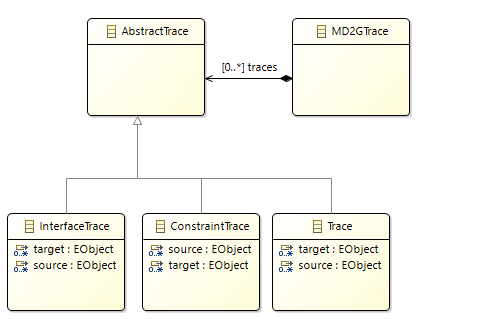
\includegraphics[keepaspectratio, width=140mm]{figures/trace-model.png}
	\caption{Trace modell EMF definíciója}
	\label{fig:trace-model}
\end{figure}


\section{A Verifikáció végrehajtása}
A verifikáció végrehajtásához két dologra van szükség. A modellnek egy leírására amit az Uppaal képes értelmezni és előállítani egy időzített automatát belőle és az Uppaal Query nyelvén megfogalmazott feltételekre. A MagicDrawToGamma kétféle lehetőséget biztosít a verifikáció végrehajtására.

\begin{enumerate}
	\item Uppaal közvetlen használata
	\item Uppaal Query Generator
	\label{en:fels}
\end{enumerate}

Első lehetőség időzített automaták leírásának előállítása amit a felhasználó megnyithat \emph{UPPAAL}-al. Ennek végrehajtása két részből áll. Először a Gamma modellt át kell alakítani, ez a \verb+StatechartToUppaalTransformer+ osztályon keresztül történik, ami a Gamma része.
\begin{lstlisting}
//initialize with a Gamma Package
StatechartToUppaalTransformer transformer = new StatechartToUppaalTransformer(p);
SimpleEntry<NTA, G2UTrace> entry = transformer.execute();
\end{lstlisting}
Ennek a kimenete két EMF alapú modell, egy \emph{trace modell} (\verb+GU2Trace+) és egy időzített autómata (\verb+NTA+). Az \textbf{időzített autómata}\footnote{a formális verifikáció az időzített autómaták formalizmusán törénik} modelljét ezután egy formális leírásként kell szerializálni amit az UPPAAL képes beolvasni. Ez a Gamma \verb+UppaalModelSerializer+ osztálya állítja elő. 
\begin{lstlisting}
//NTA, parentFolder, fileName
UppaalModelSerializer.saveToXML(entry.getKey(), selected.getPath() , name +".xml");
\end{lstlisting}
A kimenetek a \emph{Gamma Workspace-ben} az állapottérkép könyvtárába kerülnek, ahonnan a felhasználó megnyithatja őket \emph{UPPAAL}-ban.

A második lehetőség az \emph{Uppaal Query Genertor} (\ref{fig:upp-query-gen} ábra) használata. Ez egy segédablak amivel a felhasználó egy grafikus felhaszálói interfészen tud \emph{UPPAAL Query}-ket definiálni, így a felhasználónak nem szükséges elsajátítania az \emph{UPPAAL Query}-k szintaxisát.

\begin{figure}[!ht]
	\centering
	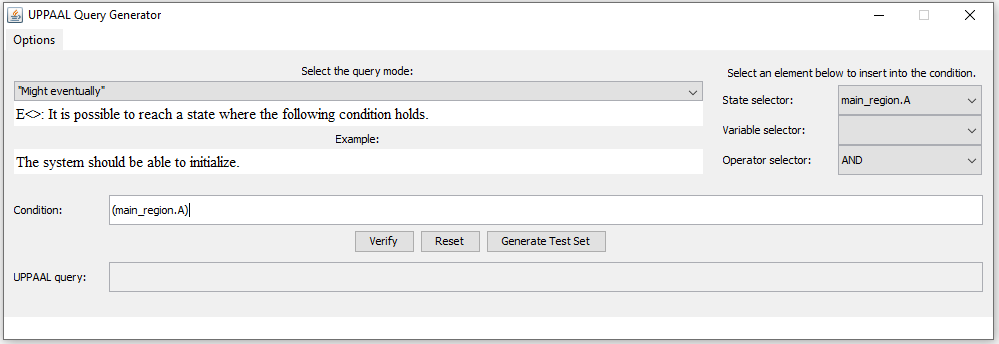
\includegraphics[keepaspectratio, width=150mm]{figures/query-gen.png}
	\caption{UPPAAL Query Generator}
	\label{fig:upp-query-gen}
\end{figure}

A Query Generátor implementációja a Gammából át lett emelve a MagicDraw plug-inba és az implementáció módosítva lett, hogy ebben a környezetben is tudjon működni. A Gamma egyik funkciója, hogy a formális verifikáció során esetleg keletkező ellenpéldákból képes teszteseteket és szimulációt generálni Yakinduhoz, ez a MagicDrawToGamma plug-in jelenlegi verziójában le van tiltva.

\section{Plulgin működés közben}

Az előző alfejezetek a MagicDrawToGamma főbb funkcióinak ismertetéséről és a funkciók megvalósítását mutatták be. Ebben az alfejezetben a  tényleges működéséről lesz szó egy példán keresztül.

\subsection{Szemléltető példa}

\paragraph{Példa specifikációja:} egy kerti világítórendszer mozgás érzékelővel van felszerelve, ha a rendszer aktív és mozgást érzékel tíz másodpercre bekapcsolja a lámpákat majd ezután kikapcsolja azokat. A rendszer inaktív állapotában nem ég egyetlen lámpa sem. 

\paragraph{Rendszer állapot alapú definíciója:} A rendszer két jól megkülönböztethető állapotból áll \verb+Acitve+ és \verb+Inactive+. Az \verb+Active+ állapot felbontható két belső állapotra, hogy égnek-e vagy sem a lámpák: \verb+LightsOn+, \verb+LightsOff+. Ezeken kívül bevezethető még két állapot, hogy érzékel-e épp mozgást a rendszer vagy sem: \verb+Idle+, \verb+Movement+. Ezek alapján a rendszer egy lehetséges leírása lehet:
\begin{figure}[H]
	\centering
	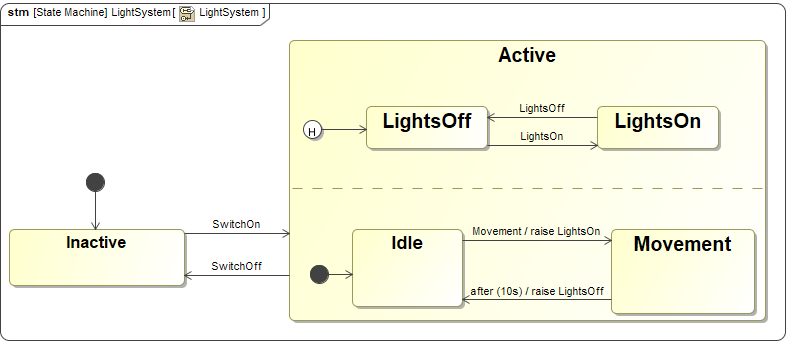
\includegraphics[keepaspectratio, width=150mm]{figures/example1.png}
	\caption{Lehetséges leírás}
\end{figure}
\subparagraph{Megjegyzés}Az egyszerűség kedvéért tekintsük, úgy hogy a folytonos mozgás során bekövetkezett \verb+LightsOn+ - \verb+LigtsOff+ - \verb+LightsOn+ váltások olyan gyorsan végbe mennek, hogy fizikailag nem képesek a lámpák lekapcsolni, hogy a villodzással ne kelljen foglalkozni


